\section{XAFS Fourier transforms}

\begin{frame} \frametitle{XAFS Fourier Transforms}

\begin{cenpage}{130mm}
Fourier Transforms are an important part of XAFS Analysis:

\begin{postitbox}{75mm}  $\displaystyle{ \chi(R) = {\rm FT}[\chi(k)] =
  \frac{1}{\sqrt{2\pi}}
  \int_{-\infty}^{\infty} { dk \, e^{i2kR} \, k^w \, \chi(k) \, \Omega(k) }} $
\end{postitbox}

\begin{itemize}
\item $\Omega(k)$ is the Window Function
\item $w$ is the $k$-weighting
\end{itemize}

\pause
\vmm
 We really use a discrete version and Fast Fourier Transform

\[
\chi(R_m) = \frac{i \delta k}{\sqrt{\pi N_{\rm fft}}}
\sum_{n=1}^{N_{\rm fft}}
e^{2\pi i n m/N_{\rm fft}} \,  k_n^w \, \chi(k_n)\, \Omega(k_n)
\]

\pause
\begin{itemize}
\item {\chik} is put on a uniform $k$-grid with spacing of  $\delta k=0.05
  {\rm\,  \AA}^{-1}$.
\item {\chik} is filled with zeros past the real data range.

\item $N_{\rm fft} = 2048$: {\chik} can go to $102.4 {\rm\, \AA}^{-1}$
  ($\sim 40\rm \, keV$) past the edge.

\item {\chir} is on a $R$-grid with spacing $\sim0.031\,\rm\AA$, and can
  go to $31.4 \,\rm\AA$.
\end{itemize}
\end{cenpage}

\end{frame}

\begin{frame} \frametitle{Fourier Transforms: Basic Properties}

  \begin{cenpage}{130mm}
Fourier Transform of a sine wave:

  \begin{tabular}{ccc}
    \begin{minipage}{55mm}
      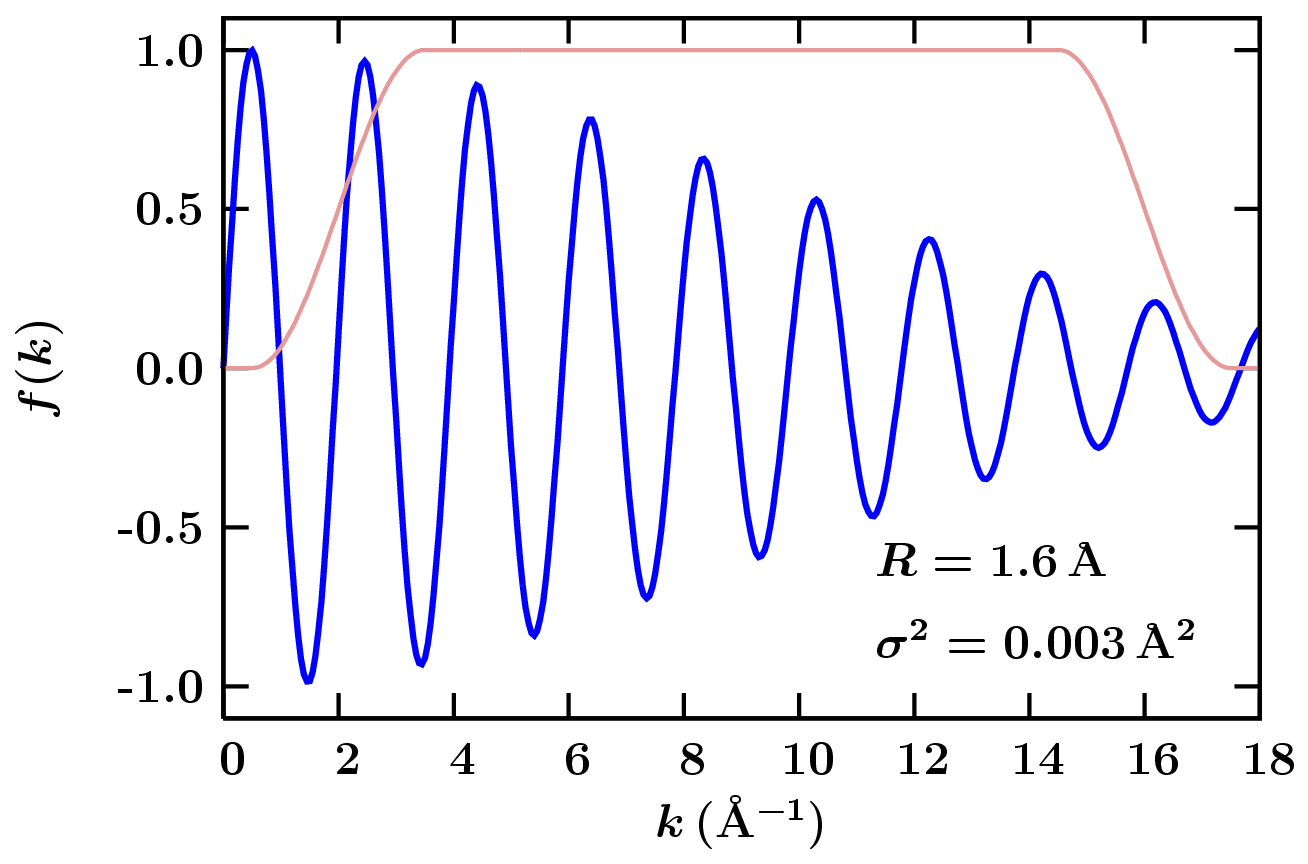
\includegraphics[width=55mm]{figs/reduction/sine_k0}
    \end{minipage}
    & $\Rightarrow $ &
    \begin{minipage}{55mm}
      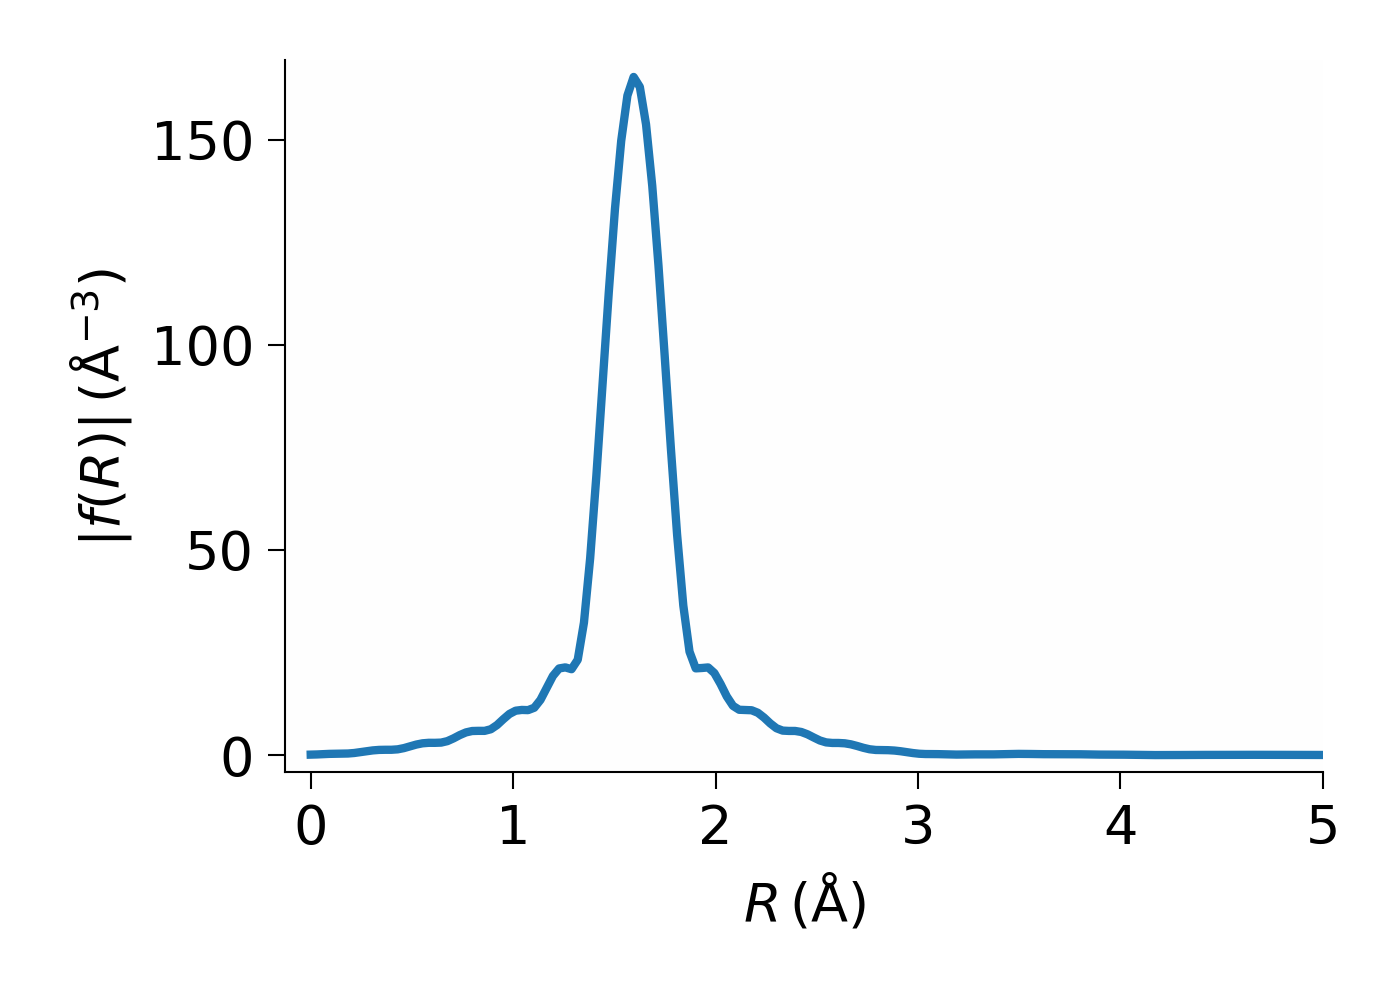
\includegraphics[width=55mm]{figs/reduction/sine_r0}
    \end{minipage}\\
    \begin{minipage}{55mm}
      \includegraphics<2->[width=55mm]{figs/reduction/sine_k}
    \end{minipage}
    & {\onslide+<2-> $\Rightarrow $}  {\onslide<1> {\vspace{40mm}}}  &
    \begin{minipage}{55mm}
      \includegraphics<2->[width=55mm]{figs/reduction/sine_r}
    \end{minipage}\\
  \end{tabular}
\end{cenpage}
\end{frame}

\begin{frame} \frametitle{Fourier Transforms: Basic Properties(2)}

  \begin{cenpage}{130mm}
Fourier Transforms are complex:

  \begin{tabular}{ccc}
    \begin{minipage}{55mm}
      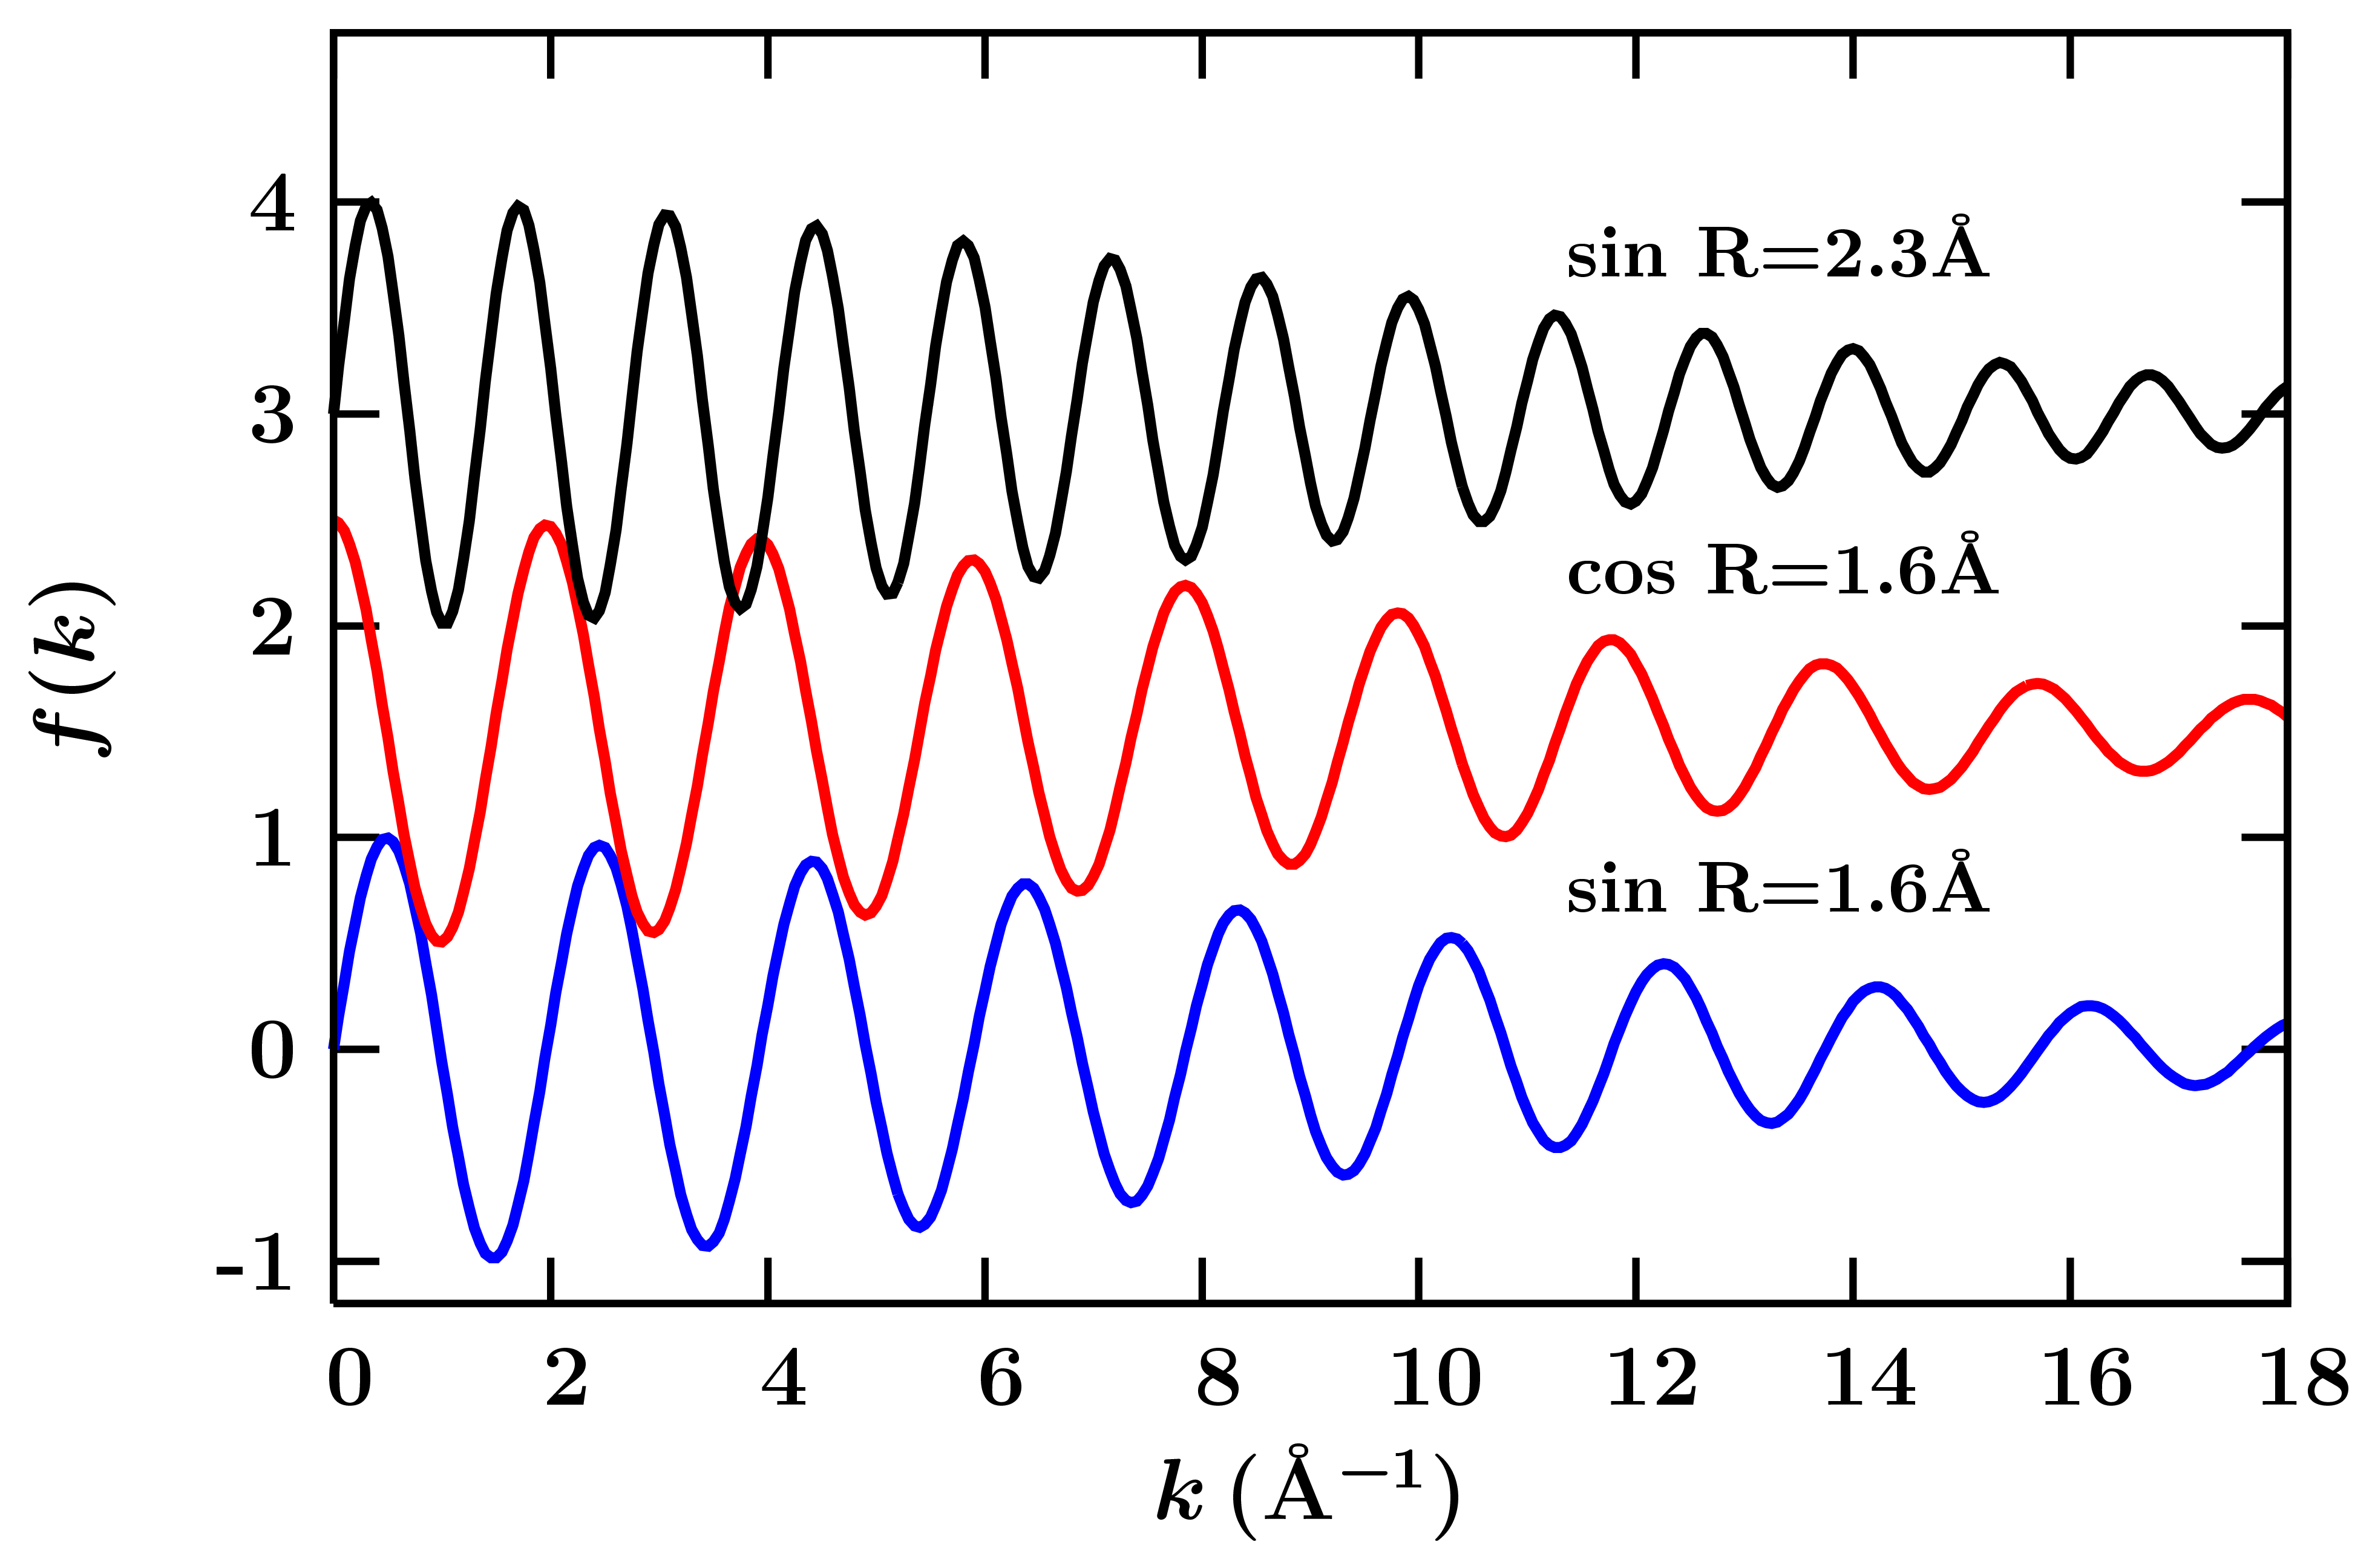
\includegraphics[width=55mm]{figs/reduction/sine_k}
    \end{minipage}
    & $\Rightarrow $ &
    \begin{minipage}{55mm}
      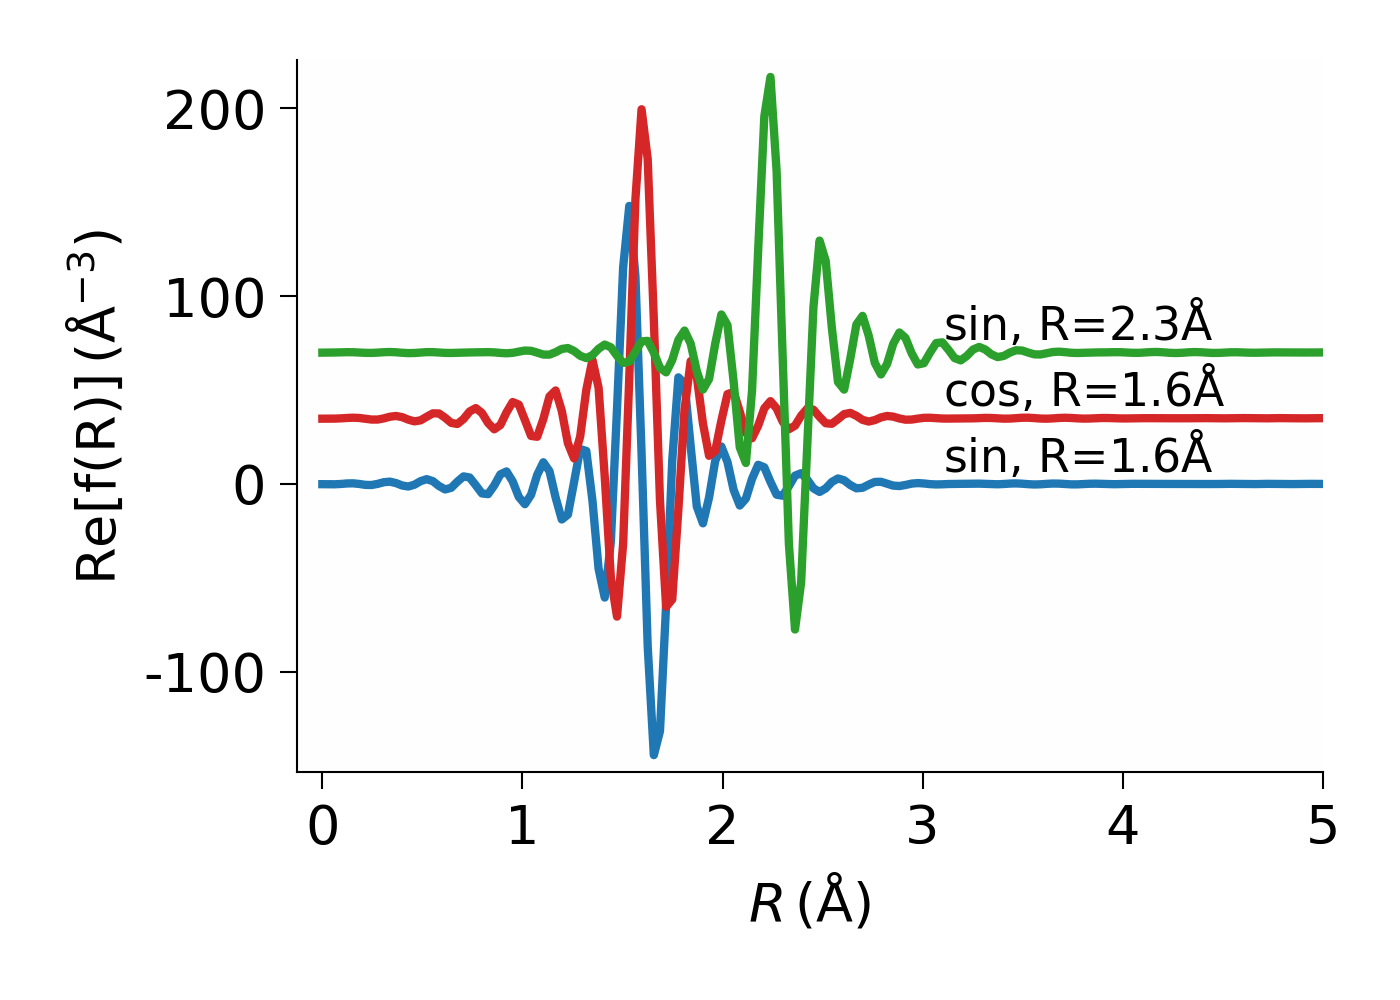
\includegraphics[width=55mm]{figs/reduction/sine_r2}
    \end{minipage}\\
    \noalign{\smallskip}
    \multicolumn{3}{l}{\onslide+<2->Waves with slightly different frequencies can cancel
      each other out, causing ``beats''  }  \\
    \noalign{\smallskip}

    \begin{minipage}{55mm}
      \includegraphics<2->[width=55mm]{figs/reduction/beat_k}
    \end{minipage}
    & {\onslide+<2-> $\Rightarrow $}  {\onslide<1> {\vspace{40mm}}}  &
    \begin{minipage}{55mm}
      \includegraphics<2->[width=55mm]{figs/reduction/beat_r}
    \end{minipage}\\

  \end{tabular}
\end{cenpage}
\end{frame}

\begin{frame} \frametitle{Fourier Transform Window Types}
\begin{cenpage}{130mm}
  \begin{tabular}{ll}
    \begin{minipage}{80mm}
      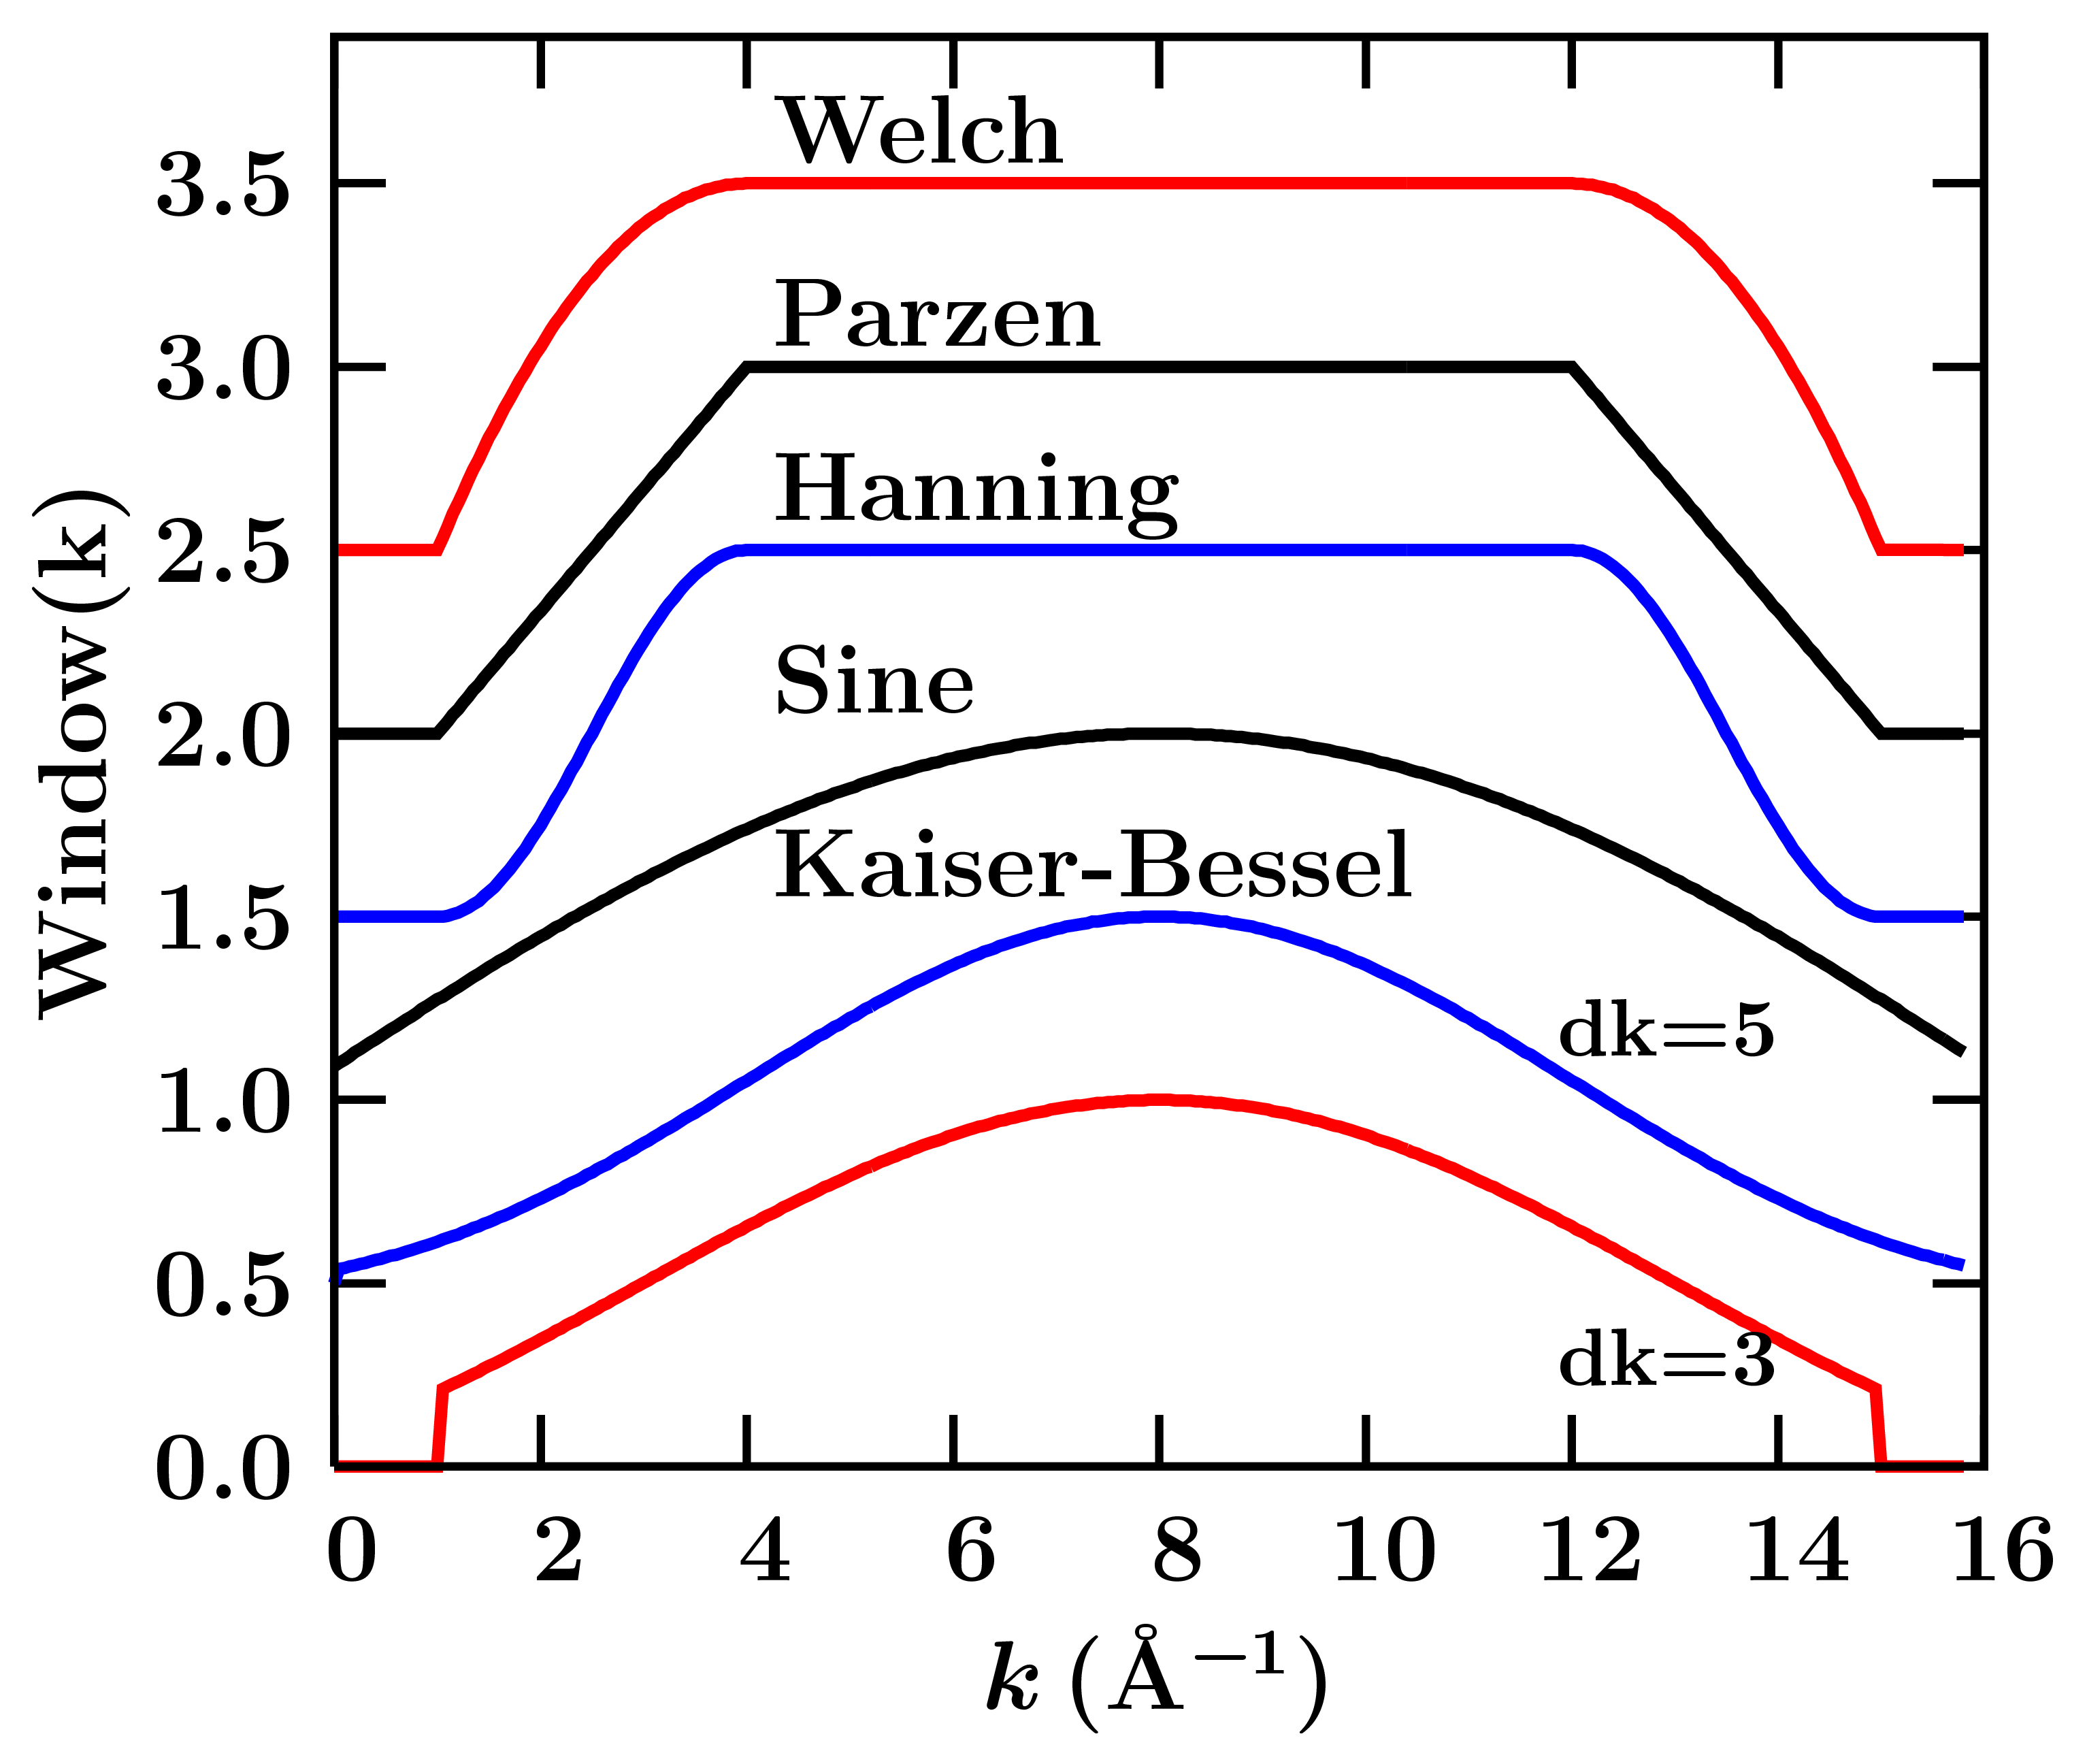
\includegraphics[width=80mm]{figs/reduction/ftwin_zoo}
    \end{minipage}
    &
    \begin{minipage}{50mm} \setlength{\baselineskip}{10pt}
      \hspace{-3mm}{\Red{Typical Window Functions}}
      \vspace{0.5mm}

      A Window Function:
      \begin{itemize}
      \item goes from 0 to 1 and back to 0
      \item $dk$ gives the width of the Window ``sill''
      \end{itemize}

      \vmm
      {\Red{Most important rule:}}

      \vmm

      Pick a window type and stick with it.

      \vmm

      Kaiser-Bessel and Hanning are the most commonly used, and recommended.

      \vmm

    \end{minipage}
  \end{tabular}

\vmm Personal Recommendation: \vmm

Kaiser-Bessel Window, $dk=4$.
\end{cenpage}
\end{frame}

\begin{frame} \frametitle{Fourier Transform Window Types}
\begin{cenpage}{130mm}

  \begin{columns}

    \begin{column}{70mm}
      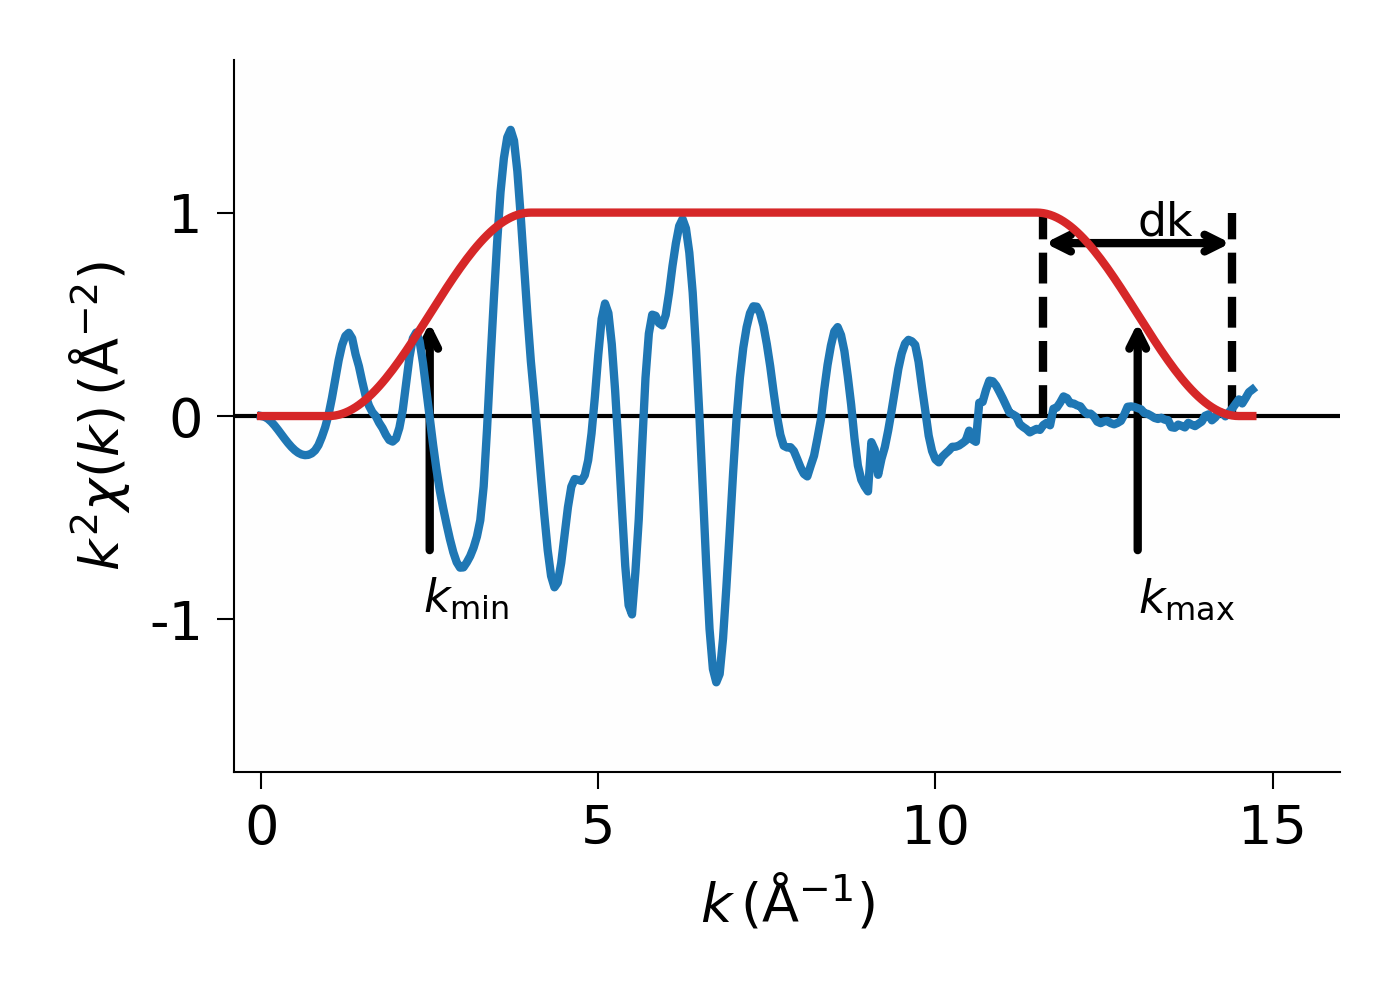
\includegraphics[width=60mm]{figs/reduction/ftwin_anat}

      \vmm
      {\onslide+<2-> {
          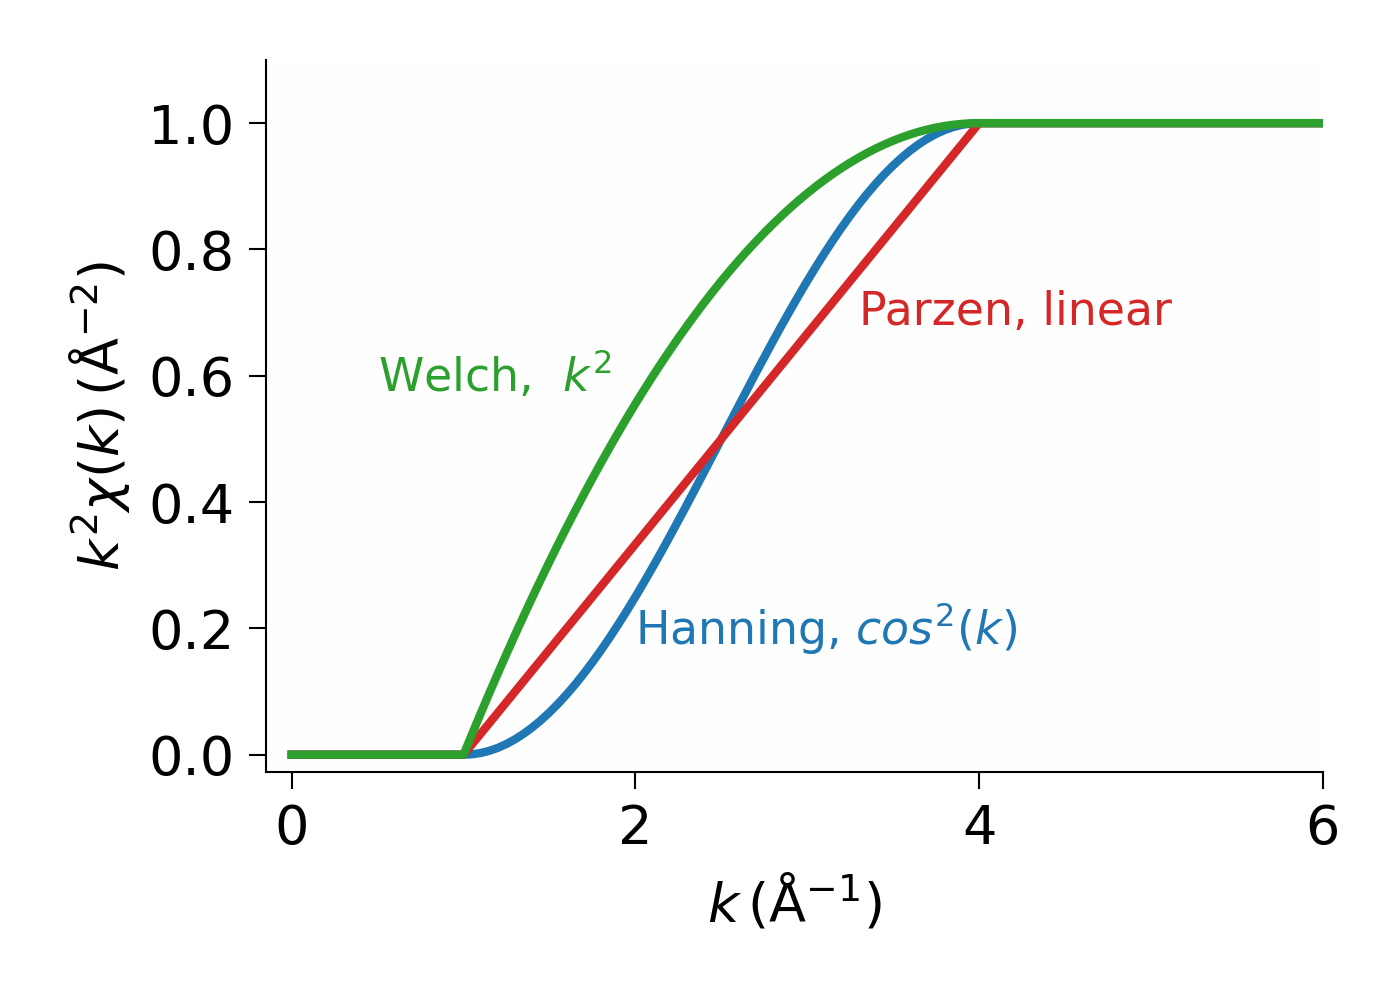
\includegraphics[width=60mm]{figs/reduction/ftwin_sills}
        }}

    \end{column}

    \begin{column}{55mm}

      \hspace{-3mm}{\Red{Fourier Window Function}}  \vspace{0.5mm}

      The meaning of $k_{\rm min}$, $k_{\rm max}$, and $dk$.

      \vspace{10mm}


      {\onslide+<2-> {

      \hspace{-3mm}{\Red{Parzen, Hanning, Welch}}

      \vspace{0.5mm}

      Details of the different Window ``sills''.

      all with $k_{\rm  min}=2\rm\,\AA^{-1}$  and $dk=3\rm\,\AA^{-1} $.

      \vspace{3mm}
    }}
    \end{column}
  \end{columns}

\end{cenpage}
\end{frame}

\begin{frame} \frametitle{Fourier Transform Window and real data}

  \begin{cenpage}{130mm}
The effect of $dk$ (for Hanning Window) and different Window Function:

  \begin{tabular}{ll}
    \begin{minipage}{60mm}
      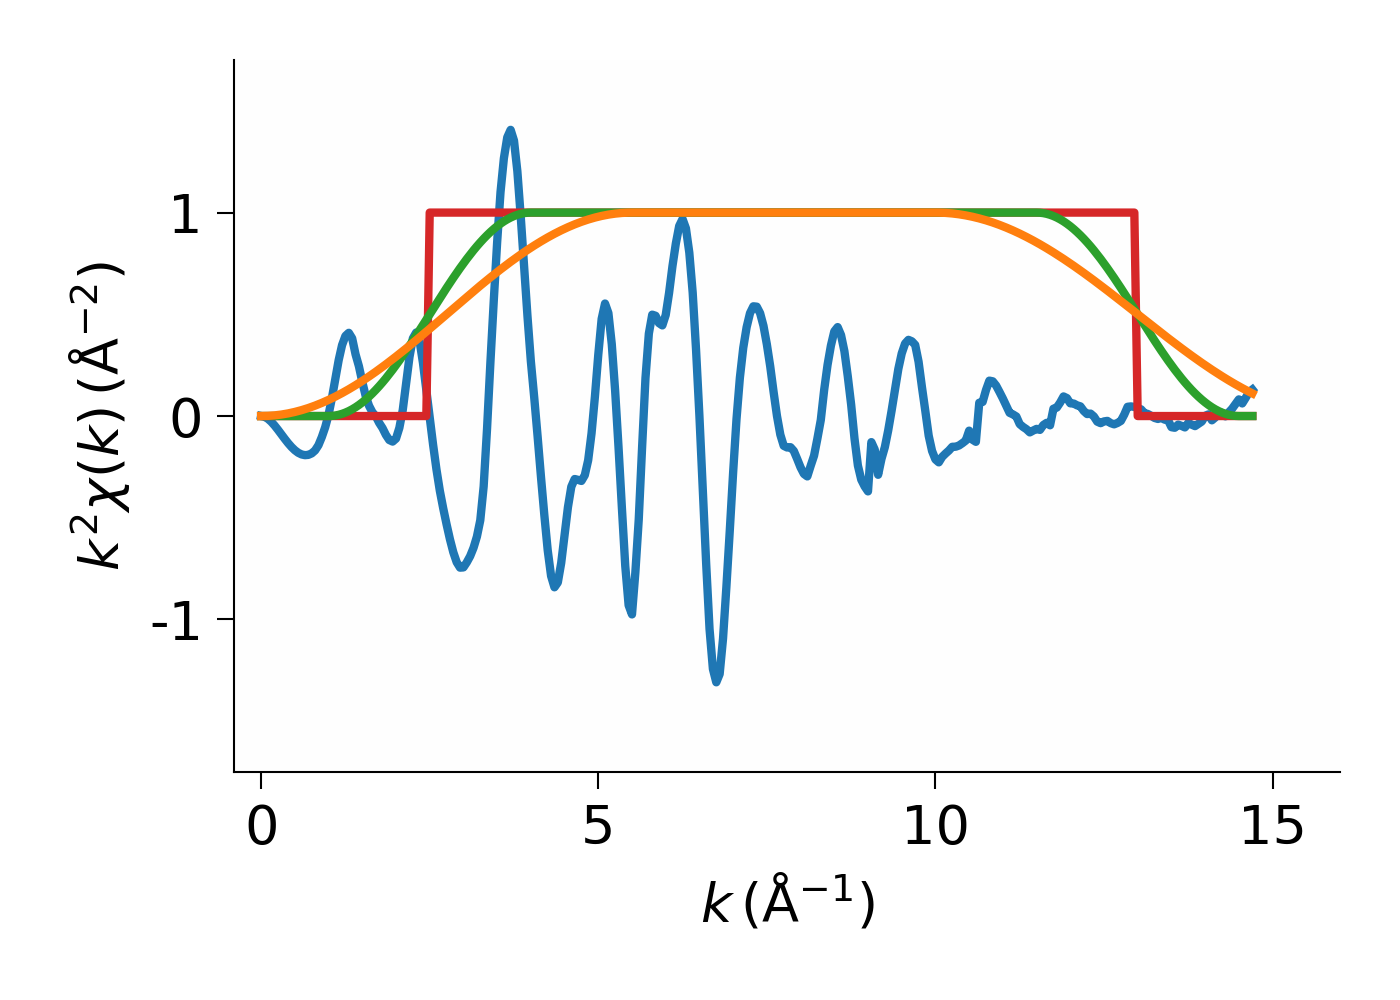
\includegraphics[width=55mm]{figs/reduction/ftwin_kdk}
    \end{minipage}
    &
    \begin{minipage}{60mm}
      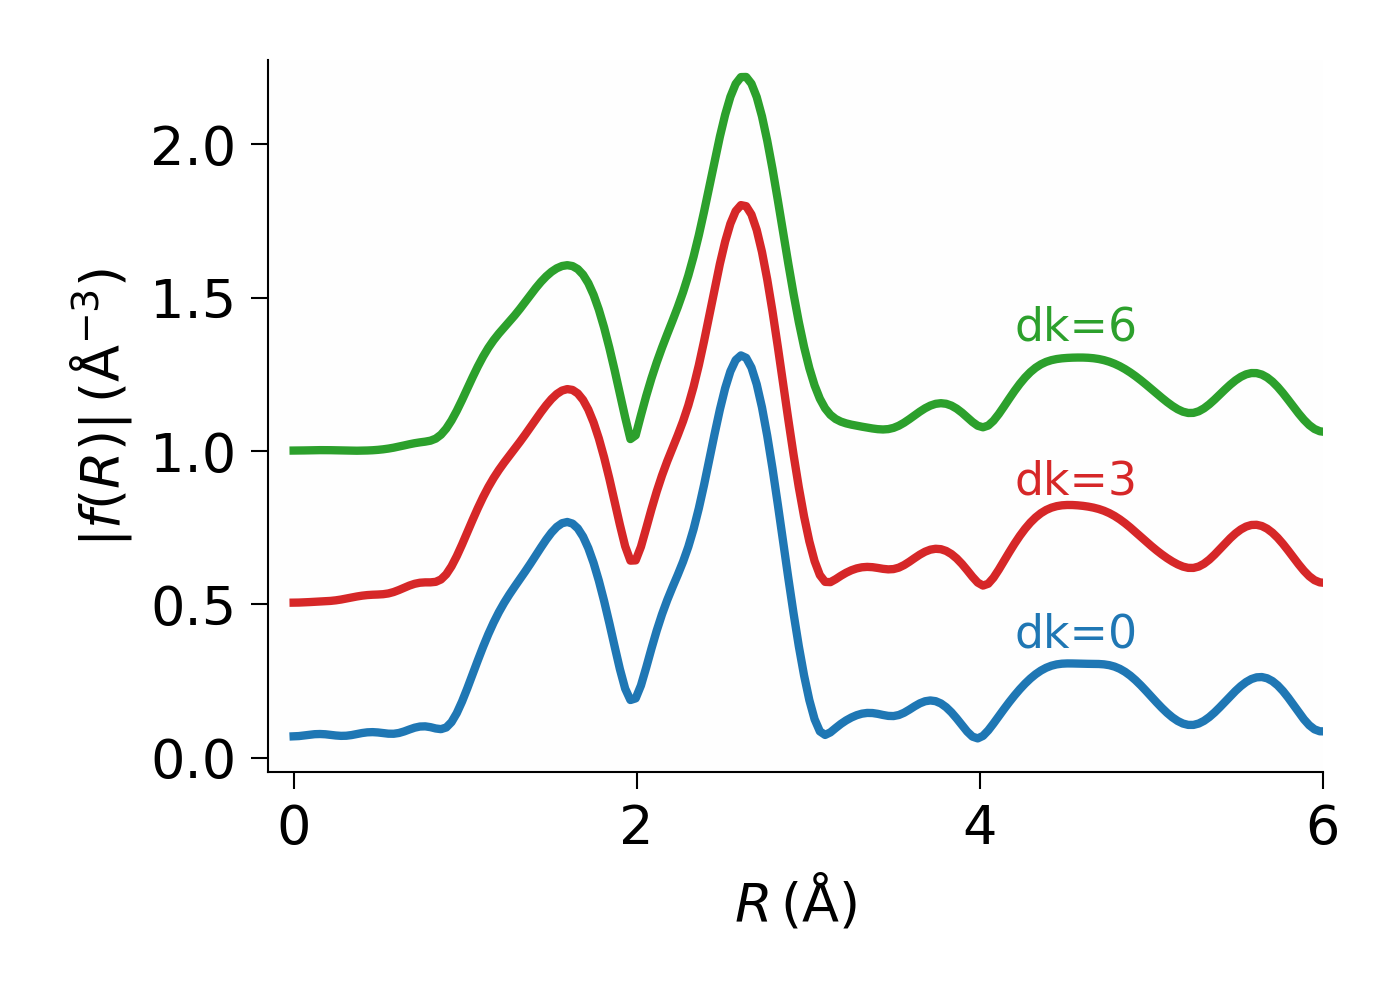
\includegraphics[width=55mm]{figs/reduction/ftwin_rdk}
    \end{minipage}\\
    \begin{minipage}{60mm}
      \includegraphics<2->[width=55mm]{figs/reduction/ftwin_wins}
    \end{minipage}
    &
    {\onslide<1> {\vspace{40mm}}}     {\onslide+<2->
      \begin{minipage}{60mm}
        Changing  $dk$ and  Window functions
        gives relatively small changes to {\chir}, most noticeable in the
       ``ringing'' of small peaks.
      \end{minipage}
    }
  \end{tabular}
\end{cenpage}
\end{frame}

\begin{frame} \frametitle{Fourier Transform Window and $k$-weight }

\begin{cenpage}{130mm}
 $\displaystyle{ \chi(R) =   \frac{1}{\sqrt{2\pi}}
  \int_{-\infty}^{\infty} { dk \, e^{i2kR} \, k^{w} \, \chi(k) \, \Omega(k) }} $

  \vmm

Changing $w$, the $k$-weighting has a significant impact:

  \vmm

  \begin{tabular}{ll}
    \begin{minipage}{65mm}
      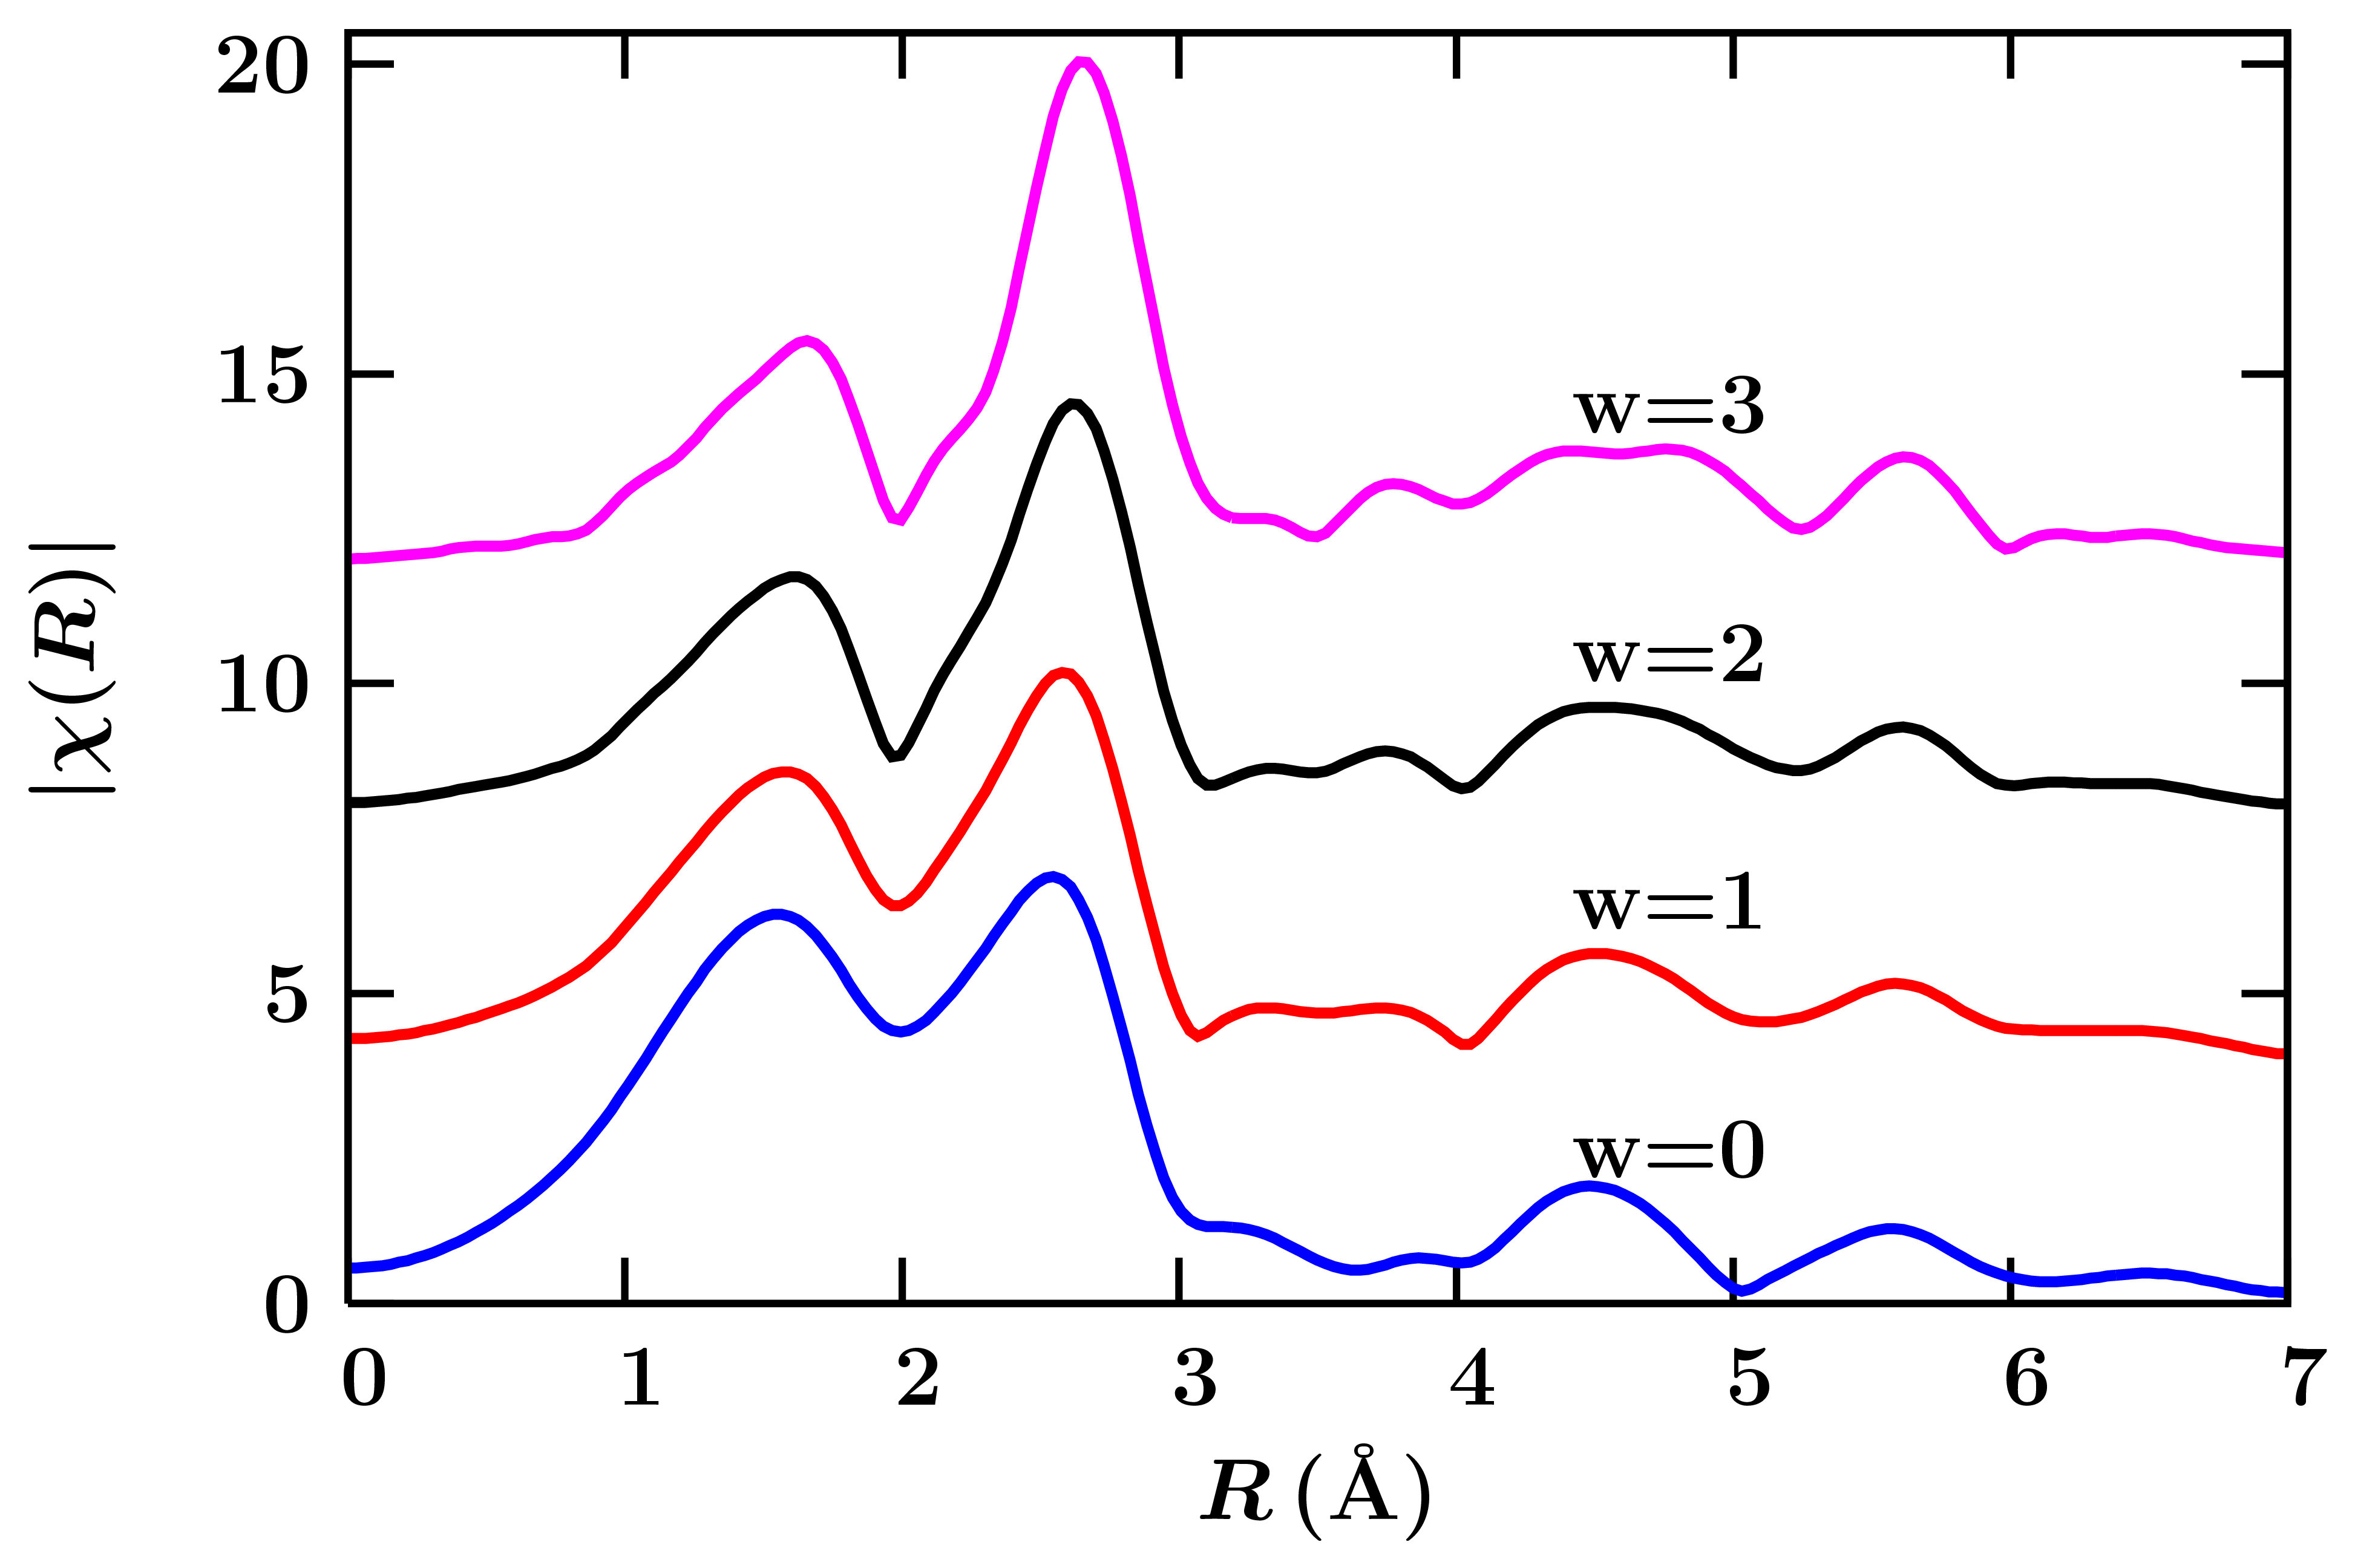
\includegraphics[width=65mm]{figs/reduction/ftwin_kw}
    \end{minipage}
    &
    \begin{minipage}{42mm}

      Fe-Fe scattering dominates with higher $w$.

      \vmm

      \vmm low $w$ emphasizes low-$k$, and low-Z scatterers.

      \vmm high $w$ emphasizes high-$k$, and  high-Z scatterers.

      \vmm
    \end{minipage}
  \end{tabular}

  \vmm This is important when trying to determine the $Z$ of a scatterer.

  \vmm Again, $w=2$ and $w=3$ are most common, and recommended.
\end{cenpage}
\end{frame}


\begin{frame} \frametitle{Fourier Transform Window and $k_{\rm min}$ }

  \begin{cenpage}{130mm}
  $k_{\rm min}$ and
  $k_{\rm max}$ are important too.

  \begin{itemize}
  \item $k_{\rm max}$ should be the end of useful data.
  \item With $k$-weight = 2, 3, it is not too important to avoid ``very low $k$''.
  \end{itemize}

  \vmm

  \begin{tabular}{ll}
    \begin{minipage}{65mm}
      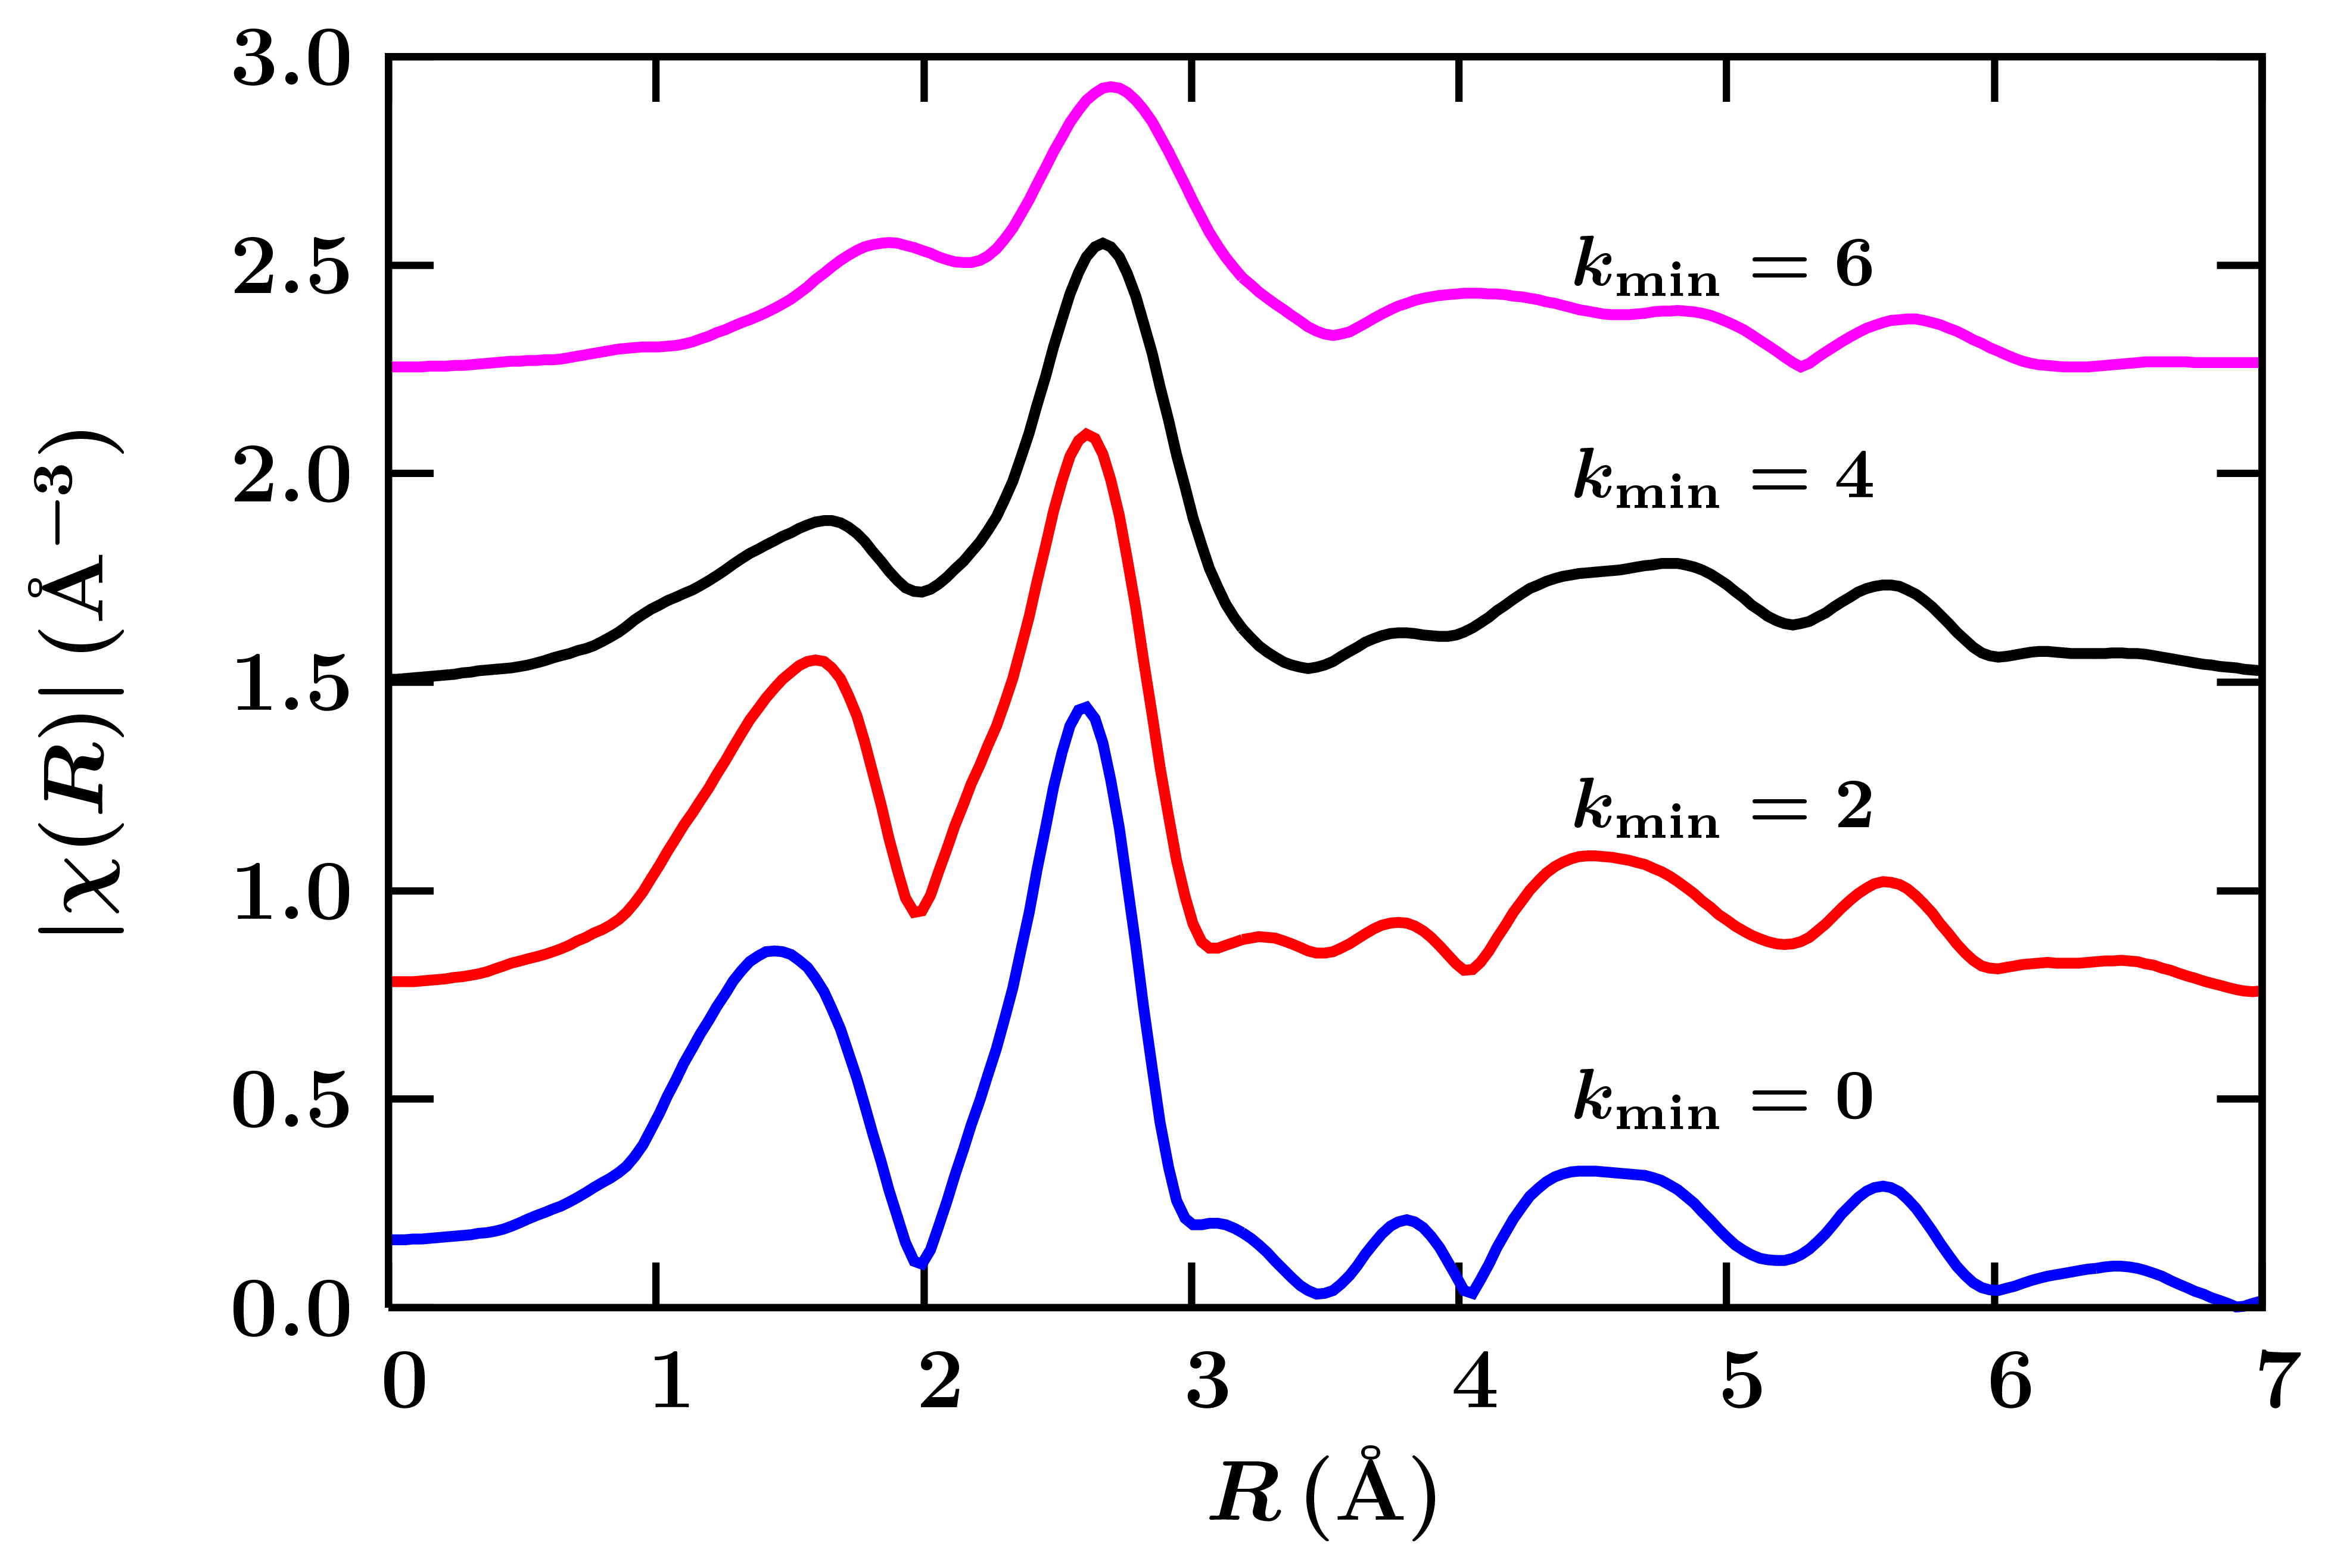
\includegraphics[width=65mm]{figs/reduction/ftwin_kmin}
    \end{minipage}
    &
    \begin{minipage}{42mm}

      Conventional wisdom:  keep $k_{\rm min} > 2\rm\,\AA^{-1}$

      \vmm
      But: don't make it too big.

      \vmm


    \end{minipage}
  \end{tabular}

\begin{center}
  \begin{postitbox}{85mm}
    Use Kaiser-Bessel with $dk=4,k_{\rm min}=2 \rm\,\AA^{-1}$

    \vmm

    Use $k$-weight=2, or 3. \hspace{10mm} Don't obsess too much.
  \end{postitbox}
\end{center}
\end{cenpage}
\end{frame}
